% !TEX encoding = UTF-8
% !TEX TS-program = pdflatex
% !TEX root = ../Tesi.tex
% !TEX spellcheck = it-IT

%************************************************

%************************************************
In questo capitolo si descriverà l'esecuzione della sperimentazione. Si partirà pertanto dai dati su cui quest'ultima è stata effettuata, proseguendo con la scelta delle modalità di esecuzione più interessanti e concludendo con una serie di tabelle e grafici contenenti i risultati ottenuti. 

\section{Decrizione del dataset}
Di seguito sono elencati i file che costituiscono il dataset. Gli esempi riportati di seguito sono stati ottenuti analizzando il sito del dipartimento di informatica di Urbana, IL: \texttt{www.cs.illinois.edu}

\subsubsection{urlsMap.txt}
Contiene la associazioni fra gli URL e il relativo codice identificativo. Questo è dovuto dalle ragioni spiegate in precedenza, ovvero ridurre i tempi di elaborazione e spazio di archiviazione. 
\\\\
\texttt{
http://cs.illinois.edu,3\\
http://cs.illinois.edu/prospective-students,4\\
http://cs.illinois.edu/current-students,5\\
http://cs.illinois.edu/courses,6\\
http://cs.illinois.edu/alumni,7\\
http://cs.illinois.edu/research,8\\
http://cs.illinois.edu/news,9\\
http://cs.illinois.edu/partners,10\\
http://cs.illinois.edu/about-us,11\\
. . .\\
}
\subsubsection{vertex.txt}
Contiene il contenuto testuale di ogni pagina esplorata. Ogni riga è quindi formata da il codice identificativo di un URL e il relativo contenuto.
\\\\
\texttt{
1	department of computer science at illinois engineering at ...\\
2	prospective students department of computer science at ...\\
3	current students department of computer science at ...\\
4	courses department of computer science at illinois ...\\
5	alumni department of computer science at illinois ...\\
6	research department of computer science at illinois    ...\\
7	news department of computer science illinois engineering ...\\
8	partners department of computer science at illinois ...\\
9	about us department of computer science at illinois ...\\
. . .\\
}
\subsubsection{edges.txt}
Questo è il file principale per la generazione delle sequenze, qui sono immagazzinate tutte le relazioni fra le pagine, ovvero gli archi che le collegano. 
\\\\
\texttt{
1	1\\
1	2\\
1	3\\
1	4\\
1	5\\
1	6\\
1	7\\
1	8\\
1	9\\
. . .\\
}
\subsubsection{sequencesIDs.txt}
Contiene le sequenze generate. I codici relativi alle pagine web sono separati da '' -1 '' e la linea finisce con un '' -2 ''. Da notare che sono riportate le sequenze che partono da un nodo casuale del grafo.
\\\\
\texttt{
137 -1 2 -1 27 -1 8 -1 52 -1 53 -1 8 -1 8 -1 10 -1 13 -1 -2\\
506 -1 5 -1 14 -1 11 -1 6 -1 2 -1 27 -1 114 -1 111 -1 11 -1 -2\\
424 -1 4 -1 12 -1 6 -1 8 -1 53 -1 4 -1 7 -1 12 -1 8 -1 -2\\
616 -1 5 -1 6 -1 8 -1 8 -1 9 -1 1 -1 21 -1 6 -1 3 -1 -2\\
51 -1 7 -1 7 -1 38 -1 38 -1 25 -1 103 -1 27 -1 113 -1 12 -1 -2\\
429 -1 10 -1 3 -1 6 -1 4 -1 11 -1 8 -1 9 -1 9 -1 3 -1 -2\\
783 -1 421 -1 5 -1 9 -1 7 -1 5 -1 2 -1 8 -1 2 -1 24 -1 -2\\
506 -1 5 -1 8 -1 52 -1 53 -1 25 -1 40 -1 13 -1 11 -1 13 -1 -2\\
638 -1 63 -1 153 -1 62 -1 63 -1 152 -1 63 -1 155 -1 13 -1 7 -1 -2\\
. . .\\
}
\subsubsection{sequencesIDsFromHomepage.txt}
Contiene le sequenze generate che partono da uno stesso nodo. La generazione di questo file avviene esplicitando il nodo di origine di ogni sequenza nella fase di generazione.
\\\\
\texttt{
1 -1 8 -1 2 -1 14 -1 2 -1 2 -1 10 -1 14 -1 66 -1 3 -1 -2\\
1 -1 18 -1 39 -1 8 -1 8 -1 24 -1 1 -1 4 -1 7 -1 25 -1 -2\\
1 -1 23 -1 -2\\
1 -1 16 -1 10 -1 3 -1 29 -1 29 -1 4 -1 25 -1 97 -1 108 -1 -2\\
1 -1 20 -1 20 -1 1 -1 11 -1 3 -1 2 -1 9 -1 10 -1 13 -1 -2\\
1 -1 25 -1 48 -1 48 -1 44 -1 42 -1 4 -1 7 -1 38 -1 38 -1 -2\\
1 -1 25 -1 115 -1 4 -1 11 -1 11 -1 1 -1 2 -1 26 -1 13 -1 -2\\
1 -1 24 -1 4 -1 9 -1 60 -1 56 -1 6 -1 25 -1 113 -1 116 -1 -2\\
1 -1 21 -1 25 -1 135 -1 32 -1 13 -1 4 -1 25 -1 149 -1 59 -1 -2\\
. . .\\
}

\section{Metodologie confrontate}
La sperimentazione si è svolta confrontando i risultati ottenuti attraverso l'applicazione di diversi algoritmi di clustering su dataset ottenuti da differenti rappresentazioni. In seguito verrano descritte le diverse rappresentazioni, i diversi algoritmi di clustering utilizzati e le metriche applicate per ottenere dei valori significativi alla valutazione.
\subsection{Partizionamento del Grafo Web}
Sono stati applicati metodologie derivanti dalla teoria dei grafi per l'estrazione di strutture connesse all'interno del grafo web. La divisione del grafo in sotto-grafi può essere effettuata seguendo diversi approcci, inoltre il grafo costruito su di un normale sito web è caratterizzato solitamente da un numero elevato di collegamenti tra pagine che indirizzano all'utilizzo di alcune tipologie di partizionamento piuttosto che altre. Infatti misure come la betweenness (ovvero il valore dato ad un arco che rappresenta quante più volte questo è attraversato nel percorrere il cammino più breve fra due nodi qualsiasi) non hanno restituito risultati significativi.
\\
L'analisi del grafo considera unicamente le relazioni che intercorrono fra le pagine web e tralascia informazioni riguardanti il contenuto.
\begin{figure}[htb]
	\centering
	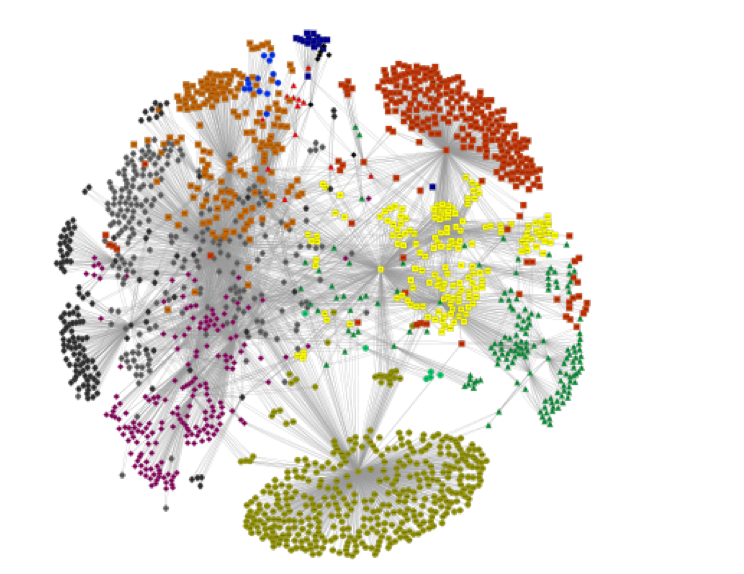
\includegraphics[width = 150mm]{graphpartitioning.png}
	\caption{Partizionamento di un grafo.}
	\label{modularity}
\end{figure}

\subsection{URL Embedding}
Considerando i random walk generati sul grafo come frasi, è possibile applicare algoritmi di word embedding per raggruppare le pagine sulla base del contesto in cui appaiono, ovvero le pagine che più verosimilmente appariranno insieme nelle sequenze di random walk. Anche questo approccio considera unicamente le relazioni fra le pagine, ma i percorsi casuali generati, considerati come frasi, raggruppano in cluster pagine che appariranno nello stesso random walk più volte, cosa che avverrà tanto più una pagina avrà collegamenti direzionati all'altra pagina. Apprendendo le rappresentazioni dai cammini invece che dal partizionamento del grafo si codificano le pagine in uno spazio vettoriale con i benefici che conseguono.

\subsection{Text Mining}
Qui viene effettuata l'analisi testuale della pagina web, utilizzando tecniche derivanti dal Text Mining. I contenuti all'interno di uno stesso sito web avranno una struttura e termini comuni, differenziandosi al variare dell'argomento trattato. La struttura gerarchica di un sito web organizza solitamente le pagine in sezioni simili. Questa metodologia tuttavia, considera solo l'informazione testuale, assumendo che i termini all'interno del sito web siano indipendenti l'uno dall'altro (cosa che nei documenti che trattano argomenti specifici non  vero) così come i documenti, ignorando le relazioni interdipendenti tra questi. Il web si discosta dall'analisi classica dei documenti proprio per le relazioni che intercorrono tra le pagine, tuttavia l'analisi testuale rimane molto importante. TFIDF

\subsection{Analisi combinata}
Dai risultati (mostrati più avanti) risulta che l'analisi singola della correlazione tra le pagine piuttosto che il contenuto testuale non bastano a codificare esaustivamente la conoscenza che una pagina web può offrire. Entrambe le informazioni sono rilevanti ed andrebbero processate combinatamente. Il vantaggio di codificare le relazioni in no spazio vettoriale offre il vantaggio di unire i vettori derivanti dagli algoritmi di word embedding con quelli derivanti dall'analisi di contenuto testuale

Se questo può essere utile nella individuazione di comunità all'interno di grafi come ad esempio social network, nelle pagine web l'informazione testuale rappresenta una parte importante e non può essere ignorata.

\subsection{Algoritmi utilizzati}
\subsubsection{WalTrap}
\subsubsection{Fastgreedy}
\subsubsection{K-Means}
\subsubsection{DBSCAN}
\subsubsection{HDBSCAN}

\section{Metriche}
\subsubsection{Silohuette}
\subsubsection{Adj rand index}
\subsubsection{V-Measure}
\subsubsection{Homogeneity}
\subsubsection{Mutual Information}



\section{Risultati ottenuti}
tabellazze

\section{Sperimentazione modulo estrazione dei perpetratori}
L'obiettivo di questa prima sperimentazione è valutare l'efficacia del sistema analizzato al fine di comprendere le cause di un eventuale successo o insuccesso delle tecniche utilizzate e quindi decidere se proseguire gli studi in questa direzione o definire strategie alternative.

La sperimentazione del sistema è stata effettuata sfruttando i dati appartenenti al database GTD (Global Terrorism Database)\cite{GTD}.
Questo database open-source, reso disponibile dal National Consortium for the Study of Terrorism and Responses to Terrorism (START), contiene informazioni su eventi terroristici avvenuti nel mondo nel periodo 1979-2011. A differenza di altri database, GTD contiene dati su incidenti terroristici nazionali e internazionali, per un totale di 104.000 istanze. Per ogni incidente sono disponibili una serie di informazioni quali data, luogo dell'incidente, armi utilizzate, numero di vittime e nomi degli individui o gruppi responsabili.
Si descrivono di seguito le caratteristiche principali del database GTD:
\begin{itemize}
	\item Contiene informazioni su 104.000 attacchi terroristici;
	\item Ad oggi la più completa base di dati non classificata di eventi terroristici avvenuti nel mondo;
	\item Include informazioni su più di 47.000 bombardamenti, 14.000 assassinii e 5300 rapimenti dal 1979 ad 2011;
	\item Contiene per ogni caso almeno 45 variabili, fino ad arrivare a 120 variabili nel caso di incidenti recenti;
	\item Supervisionato da un gruppo consultivo di 12 esperti in campo terroristico;
	\item Oltre 3.500.000 articoli di news e 25.000 sorgenti di news sono stati analizzati per raccogliere dati sugli incidenti avvenuti nel solo periodo 1998-2011.
\end{itemize}

Per la sperimentazione sono stati selezionati 10732 istanze (ognuna associata a uno su 50 distinti nomi di perpetratori), da cui sono state estratti la descrizione testuale dell'incidente terroristico (news), la data associata all'evento, titolo dell'articolo e il nome dei perpetratori, utilizzati per popolare il database di TB-CREDIS. 
Delle 10732 istanze solo 7361 sono utilizzate per l'estrazione delle entità nominali (per un totale di 44 nomi di perpetratori), in quanto la descrizione testuale delle istanze eliminate non conteneva il nome dei perpetratori, quindi sarebbe stato impossibile per qualsiasi Named Entity Recognizer individuare le entità corrette.

\paragraph{} Tratteremo di seguito come valutare un sistema di Entity Extraction, in modo da verificare se il sistema realizzato ha prodotto risultati significativi. 

In generale la valutazione dei sistemi di machine learning è effettuata sperimentalmente piuttosto che analiticamente. Questa infatti non può essere formalizzata (a causa della sua natura soggettiva) e quindi non può essere valutata analiticamente.
La valutazione sperimentale solitamente misura l'efficacia di una sistema, ossia l'abilità nel prendere la giusta decisione. Questa viene
misurata in termini di \textit{precisione} (precision) e  \textit{richiamo} (recall).
In particolare, definite le seguenti misure:
\begin{itemize}
	\item \textbf{True Positive}: entità correttamente etichettate 
	
	
	(\textit{President \textbf{Bush} attended the ceremony});
	\item \textbf{True Negative}: termini correttamente non etichettati come positivi 
	
	(\textit{ \texttt{President} \textbf{Bush} attended the ceremony})
	\item \textbf{False Positive}: termini non entità, erroneamente etichettati come tali
	
	(\textit{President \textbf{Bush} attended the \textbf{ceremony} })
	\item \textbf{False Negative}: entità erroneamente non etichettate come tali
	
	(\textit{President Bush attended the ceremony.})
\end{itemize}
è possibile calcolare una stima della precisione (ossia il numero di entità correttamente etichettate sul numero totale di entità individuate), richiamo (ossia il numero di entità correttamente etichettate rispetto a tutte le entità presenti) e F-Score (che permette di definire un buon trade-off tra precisione e richiamo) del sistema:
\begin{equation}
\label{recall}
Recall= \frac{True Positive}{(True Positive + False Negative)};
\end{equation}
\begin{equation}
\label{precision}
Precision= \frac{True Positive}{(True Positive + False Positive)};
\end{equation}
\begin{equation}
\label{Fscore}
F-Score= \frac{2(Precision * Recall)}{(Precision + Recall)};
\end{equation}

Praticamente, per ottenere queste misure è possibile procedere in due modi:
\begin{itemize}
	\item Micro-Media, i valori delle misure sono valutati localmente alle classi e poi mediati sul loro numero per ottenere una stima globale delle
prestazioni del sistema;
	\begin{equation}
	 Precision= \frac{TP}{TP+FP}= \frac{\sum_d TP_{d}}{\sum_d (TP_d+FP_d)}
	\end{equation}

	\begin{equation}
	 Recall= \frac{TP}{TP+FN}= \frac{\sum_d TP_{d}}{\sum_d (TP_d+FN_d)}
	\end{equation}
	dove $TP_d, FP_d$ e $FN_d$ sono rispettivamente il numero di entità positive correttamente etichettate (TP), il numero di termini erroneamente etichettati come entità (FP) e il numero di entità non etichettate come tali (FN) per il generico documento $d$ appartenente alla collezione.
	\item Macro-Media, la precisione e il richiamo sono prima valutate localmente per ogni documento $d$ e poi globalmente dalla media dei risultati:
	
	\begin{equation}
	Precision= \frac{\sum_d Precision_d}{|Documents|}
	\end{equation}
	
	\begin{equation}
	Recall= \frac{\sum_d Recall_d}{|Documents|}
	\end{equation}
\end{itemize}
dove $Documents$ è l'insieme dei documenti appartenenti alla collezione, mentre $Precision_d$ e $Recall_d$ sono la precisione e il richiamo calcolati sul documento $d \in Documents$.


Per valutare le prestazioni del sistema realizzato, i risultati ottenuti verranno confrontati con la precisione e il richiamo calcolati sul solo sistema di Named Entity Extraction(NER), che verrà quindi utilizzato come baseline. 
Per l'estrazione delle entità verranno utilizzati i tool TextPro e LingPipe, mentre per la creazione dell'albero delle dipendenze verrà utilizzato Stanford Parser. 
Per ogni documento verranno calcolate le misure precedentemente definite utilizzando la seguente strategia.

Per ogni documento:
\begin{itemize}
\item \textbf{True Positive}=1 se il sistema ha restituito almeno 1 volta il perpetratore, 0 altrimenti;
\item \textbf{False Negative}=1 se il sistema non ha mai restituito il perpetratore, 0 altrimenti;
\item \textbf{False Positive} = numero di entità estratte - numero di entità perpetratici.
\end{itemize}


Calcolati i True Positive, False Positive, True Negative, False Negative si realizza il calcolo della precisione e richiamo tramite micro-media.
Si riportano pertanto le caratteristiche hardware e software utilizzate per questa sperimentazione:
\begin{itemize}
	\item CPU Intel Core i5 2500K - Core: 4 - Frequenza: 4Ghz;
	\item RAM 8GB DDR3 1600Mhz;
	\item Hard Disk Western Digital 500GB 5400rpm;
	\item S.O. Microsoft Windows 7 64bit;
	\item DBMS PostgreSQL 9.2;
	\item TextPro 1.4;
	\item LingPipe Royalty Free;
	\item Wordnet 2.1;
	\item Strawberry Perl (64-bit) 5.16.2.1;
	\item Java 1.7 update 9 - 64bit.
\end{itemize}

Per rendere compatta la presentazione dei risultati, saranno utilizzate le seguenti abbreviazioni:
\begin{itemize}
\item \textbf{TPner} = Named Entity Extraction realizzata con TextPro;
\item \textbf{LPner} = Named Entity Extraction realizzata con LingPipe;
\item \textbf{TP+Stanford} = estrazione delle entità realizzata con TPner e selezione dei perpetratori attraverso Stanford Parser;
\item \textbf{LP+Stanford} = estrazione delle entità realizzata con TPner e selezione dei perpetratori attraverso Stanford Parser;
\end{itemize}
Infine si riportano di seguito le tabelle e i grafici dei risultati ottenuti:
\begin{table}[H]
	\centering
	\footnotesize
	\begin{tabular}{|cccc|}
	\hline
	\textbf{Metodo}  & \textbf{Precisione} & \textbf{Richiamo} & \textbf{F-Score} \\ \hline
	TPner & 0,6 & 0,83 & 0,70\\ 
	LPner & 0,52 & 0,85 & 0,65\\ 
	TP+Stanford & 0,86 & 0,87 & 0,86\\ 
	LP+Stanford & 0,72 & 0,76 & 0,74\\ 
	\hline
	\end{tabular}
	\caption{Risultati sperimentazione estrazione perpetratori}
	\label{tabConfrontoRis}
\end{table}

Osservando la figura \ref{figConfrontoRis} e la tebella \ref{tabConfrontoRis} è possibile notare come la precisione e il richiamo maggiori sono ottenuti combinando le informazioni estratte da TextPro con le dipendenze sintattiche calcolate da Stanford Parser (precisione=86\%, richiamo=87\%).

Poiché il confronto tra le entità estratte dal Named Entity Recognizer e quelle estratte dal Dependencies Analyzer è realizzato tramite string matching è possibile che molte corrispondenze corrette vengano perse a causa di errori ortografici o tipografici.
Per esempio, dato il documento:

\textit{``A suicide bomber wounded two police officers and a bystander as he approached a police station in Diyarbakir, Turkey. The Kurdistan Worke?s Party (PKK) was suspected of this attack.''}, associato all'organizzazione criminale \textit{``Kurdistan Worke's Party''},

i sistemi Named Entity Recognizer e Dependencies Analyzer riconoscono la stringa ``Kurdistan Worke?s Party'' come entità perpetratrice, ma poichè non esiste un matching perfetto tra ``Kurdistan Worke's Party'' e ``Kurdistan Worke?s Party'' l'entità estratta è scartata dalla lista delle entità corrette.
Per risolvere questo problema, e quindi migliorare il richiamo dei sistemi, è possibile utilizzare funzioni di matching che verifichino l'esistenza di una corrispondenza parziale tra le entità predefinite e quelle estratte \cite{Deng12}.
Un altro problema da affrontare per migliorare la qualità dei risultati prodotti è rappresentato dall'esistenza di possibili gerarchie tra le entità criminali predefinite. 
Per esempio il dataset analizzato contiene come entità perpetratrici le organizzazioni ``Al-Qa`ida'', ``Al-Qa`ida in the Arabian Peninsula (AQAP)'', ``Al-Qa`ida in Iraq'', che sono caratterizzate da relazioni di tipo gerarchico. In questo caso il calcolo delle misure True Positive, False Positive, True Negative e False Negative, come precedentemente definito, non risulta appropriato in quanto gli errori di estrazione non hanno tutti pari importanza, ma  si possono distinguere errori \textit{più gravi}, consistenti  nell'estrazione di entità che non sono correlate gerarchicamente con quella di effettiva appartenenza, ed errori \textit{meno gravi} in cui le entità estratte sono correlate gerarchicamente rispetto a quella effettiva.

\section{Sperimentazione predizione attività criminali}
Per quanto riguarda la sperimentazione della seconda componente realizzata si è deciso di utilizzare dati generati artificialmente. Nel processo di generazione sono state fatte determinate assunzioni e si è dovuto tenere conto di alcuni fattori. 

In particolare, sono stati considerati i seguenti obiettivi:
\begin{itemize}
	\item individuazione di un insieme di finestre temporali di ampiezza plausibile, relativamente ai fenomeni che si stanno analizzando;
	\item definizione di un insieme di criminali;
	\item per ciascuno di essi, generazione di un insieme di documenti relativi ad un particolare argomento (crimine), con data/ora appartenente ad una delle finestre temporali definite;
	\item definizione di alcune evoluzioni nel tempo.
\end{itemize}

Riguardo alle finestre temporali, poiché i fenomeni che si immagina di analizzare sono piuttosto lenti, si è deciso di porre l'ampiezza ad 4 anni e di rappresentare il periodo 1970-2009 (tabella \ref{TAB_FinestreTemporali}).
\begin{table}[htb]
	\centering
	\footnotesize
	\begin{tabular}{|cccc|}
	\hline
	\textbf{tw\_id} & \textbf{tw\_name} & \textbf{tw\_start\_date} & \textbf{tw\_end\_date} \\ \hline
	1 & 1970-1973 & 1970-01-01 00:00:00 & 1973-12-31 23:59:59 \\
	2 & 1974-1977 & 1974-01-01 00:00:00 & 1977-12-31 23:59:59 \\
	3 & 1978-1981 & 1978-01-01 00:00:00 & 1981-12-31 23:59:59 \\
	4 & 1982-1985 & 1982-01-01 00:00:00 & 1985-12-31 23:59:59 \\
	5 & 1986-1989 & 1986-01-01 00:00:00 & 1989-12-31 23:59:59 \\
	6 & 1990-1993 & 1990-01-01 00:00:00 & 1993-12-31 23:59:59 \\
	7 & 1994-1997 & 1994-01-01 00:00:00 & 1997-12-31 23:59:59 \\
	8 & 1998-2001 & 1998-01-01 00:00:00 & 2001-12-31 23:59:59 \\
	9 & 2002-2005 & 2002-01-01 00:00:00 & 2005-12-31 23:59:59 \\
	10 & 2006-2009 & 2006-10-01 00:00:00 & 2009-12-31 23:59:59 \\
	\hline
	\end{tabular}
	\caption{Finestre temporali definite.}
	\label{TAB_FinestreTemporali}
\end{table}

Riguardo ai criminali, non essendo interessati ad identificarli personalmente, è possibile generarne un numero a piacimento, assegnando un identificatore numerico progressivo a ciascuno di essi.

La problematica fondamentale risiede nella generazione dei documenti, la quale non deve descrivere una situazione troppo banale ma, allo stesso tempo, neanche troppo particolare. Si è deciso di individuare un insieme di argomenti, ciascuno dei quali rappresentati da alcuni termini chiave:

\begin{itemize}
	\item \textbf{omicidio:} \emph{homicide, weapon, pistol, shotgun, gun, blood, dead, handgun, victim, knife, bullet, murder, assassin, killer};
	\item \textbf{droga}: \emph{drug, cocaine, heroine, hashish, traffic, import, hide, overdose, psychoactive, hallucinogen, ketamine};
	\item \textbf{corruzione:} \emph{corruption, money, contract, politic};
	\item \textbf{estorsione:} \emph{extortion, money, violence, organized, weapon, commercial};
	\item \textbf{pedofilia:} \emph{pedophilia, child, young, rape, sexual, porn, violence};
	\item \textbf{stupro:} \emph{rape, sexual, violence, blood};
	\item \textbf{rapina-furto:} \emph{robbery, rapine, weapon, money, steal, theft}.
\end{itemize}

In totale sono state previste dunque 7 tipologie di crimini. Una delle difficoltà che il sistema si trova ad affrontare è dunque quella di riuscire a differenziare tra le diverse tipologie, considerando la presenza di termini in comune a più argomenti, la presenza di termini non propriamente specifici di atti criminali (es. \emph{money, traffic}) e la differente quantità di termini che descrivono gli argomenti. Oltre ai termini specifici, i documenti sono stati completati da una serie di termini presi casualmente da un vocabolario (termini rumore). 

In generale, nella generazione dei documenti si è tenuto conto dei seguenti fattori: 
\begin{itemize}
	\item la quantità, per ciascun criminale;
	\item la lunghezza, quantificabile in numero di parole;
	\item l'argomento, che deve riguardare una delle 7 tipologie di crimine previste;
	\item la collocazione temporale.
\end{itemize}
Per la sperimentazione si è deciso di definire 4 dataset generati a partire da 500 criminali di Training e 100 di Test, ciascuno con al massimo 100 documenti associati, aventi data compresa tra l'1 Gennaio 1970 e il 31 Dicembre 2009. La probabilità per i criminali di Training di comparire in una delle 10 finestre temporali precedentemente definite è pari al 90\%, mentre i criminali di Test compariranno in tutte le finestre temporali.
 
Si riporta di seguito l'algoritmo generale.
\footnotesize
\begin{algorithm}[H]
\caption{Generazione dei documenti}
\begin{algorithmic}

	\State $numCrim\gets 600$;	\Comment{Numero di criminali da generare in totale}
	\State $numCrimTraining\gets 500$ \Comment{Numero di criminali di Training da generare}
	\State $numDocs\gets 100$;	\Comment{Numero massimo di documenti per ciascun criminale}
	\State $biasPercentage\gets 0.7$;	\Comment{Probabilità che un criminale commetta la stessa tipologia di crimini della finestra temporale precedente}
	\State $criminalTrainingProb\gets 0.9$;	\Comment{Probabilità che un criminale di Training abbia documenti in una finestra temporale}
	\State $criminalTestProb\gets 1$;	\Comment{Probabilità che un criminale di Test abbia documenti in una finestra temporale}
	\State $n$	\Comment{Numero di finestre temporali definite. In questo caso è pari a 10.}
	\State $topics$ \Comment{Insieme degli argomenti.}
 	
 	\vspace*{+1cm}
 	
	\State \textbf{Begin}
	\For{$i = 1 \to numCrim$} 
		\State $crim\gets generateCriminal()$;
		\ForAll{timewindows tw}
		\State $topic \gets \Call{randomSelectTopic}{topics, biasPercentage}$; 
		\If{$i\leq numCrimTraining$}
			\State $numDocsTw \gets \Call{random}{0, numDocs/n, criminalPresentProb}$; 
		\Else
			\State $numDocsTw \gets \Call{random}{0, numDocs/n, criminalTestProb}$;
		\EndIf
			\For{$j = 1 \to numDocsTw$}
				\State $doc\gets$ \Call{generateDoc}{topic};
				\State \Call{associateDocument}{crim, doc};
			\EndFor
		\EndFor 
	\EndFor
	\State \textbf{End}
\end{algorithmic}
\end{algorithm}
\newpage
\normalsize
dove:
\begin{itemize}
	\item \emph{randomSelectTopic (topics, biasPercentage)} sceglie casualmente un argomento tra i 7 disponibili, ma con probabilità pari a \emph{biasPercentage} sceglie quello della finestra temporale precedente;
	\item \emph{random(0, numDocs/n, criminalPresentProb)} estrae un numero casuale tra 0 e \emph{numDocs/n} con probabilità \emph{criminalPresentProb};
	\item \emph{generateDoc(topic)} genera un documento relativo al topic fornito, seguendo l'algoritmo di seguito riportato.
\end{itemize}

\footnotesize
Siano:
\begin{algorithmic}
	\State $minNumWordsDoc\gets 1500$; \Comment{Numero minimo di parole rumore nel documento}
	\State $maxNumWordsDoc\gets 2000$; \Comment{Numero massimo di parole rumore nel documento}
			
	\State $topicWordMinOcc\gets 10$;	\Comment{Numero minimo di occorrenze per una parola chiave}
	\State $topicWordMaxOcc\gets 15$;	\Comment{Numero massimo di occorrenze per una parola chiave}
	\State $dictWordMinOcc\gets 1$;	\Comment{Numero minimo di occorrenze per una parola rumore}
	\State $dictWordMaxOcc\gets 3$;	\Comment{Numero massimo di occorrenze per una parola rumore}
	\State $topicWordsPercentage\gets 0.6$;	\Comment{\% di parole chiave inserite dell'argomento scelto}
	\State $listWordsTopic$ \Comment{Parole chiave associate all'argomento}
	\State $listWordsDict$ \Comment{Parole comuni del dizionario (rumore)}
	\State $numWordsTopic$ 
	{Numero di parole chiave associate all'argomento}
\end{algorithmic}\ 
\begin{algorithmic}
	\State \textbf{Begin}
	\State $doc\gets emptyDocument();$
	\State $numWords\gets random(minNumWordsDoc, maxNumWordsDoc);$
	\For{$i = 1 \to numWords$}
		\State $word\gets randomSelectWord(listWordsDict);$
		\State $removeWord(listWordsDict, word);$
		\State $numOcc\gets random(dictWordMinOcc, dictWordMaxOcc);$ 
		\For{$j = 1 \to numOcc$}
			\State $addWord(doc, word);$
		\EndFor
	\EndFor
	
	\State $numWords\gets topicWordsPercentage*numWordsTopic;$
	\For{$i = 1 \to numWords$}
		\State $word\gets randomSelectWord(listWordsTopic);$
		\State $removeWord(listWordsTopic, word);$
		\State $numOcc\gets random(topicWordMinOcc, topicWordMaxOcc);$ 
		\For{$j = 1 \to numOcc$}
			\State $addWord(doc, word);$
		\EndFor
	\EndFor
	
	\Return doc;
	
	 \textbf{End}
\end{algorithmic}
\normalsize
Il trattamento riservato alle parole chiave è dunque il medesimo di quelle rumore, fatta eccezione per la frequenza più elevata (tra 10 e 15 anziché tra 1 e 3).

Seguendo tale strategia, sono stati generati artificialmente 4 dataset cosi composti:
\begin{table}[H]
	\centering
	\footnotesize
	\begin{tabular}{|cccc|}
	\hline
	\textbf{\#} & \textbf{DB\_Name} & \textbf{\# Criminali di Training} & \textbf{\# Criminali di Test} \\ 
	\hline
	1 & DB\_Completo & 600 & 0 \\
	2 & DB\_Test1 & 590 & 10 \\
	3 & DB\_Test2 & 550 & 50 \\
	4 & DB\_Test3 & 500 & 100 \\
	\hline
	\end{tabular}
	\caption{Data Set su cui effettuare la sperimentazione.}
	\label{TAB_DB}
\end{table}
Per ogni criminale appartenente all'insieme di Test verranno eliminati i documenti le cui date rientrano nei periodi 1982-1985,1994-2001 (ossia nelle finestre con Id 4,7,8).
Una volta generati i dati, si è reso necessario individuare le modalità di esecuzione, in quanto il sistema prevede diverse fasi, ciascuna delle quali
eseguibile con diverse metodologie e con diversi parametri. Le combinazioni possibili risultano praticamente infinite, pertanto sono state fatte delle scelte al fine di ridurle ad un numero accettabile: 
\begin{itemize}
\item \textbf{Feature Selection}: selezione dei 30 termini con maggior varianza.
\item \textbf{Calcolo posizione semantica dei criminali}: MaxDensity con parametri SIGMA = 0.05, h (numero finestre passate da considerare) = 5;
\item \textbf{Clustering}: K-Means con stima del parametro k (numero di cluster da generare) = 7, pari cioè al numero di cluster realmente esistenti;
\item \textbf{Calcolo della posizione semantica dei cluster}: calcolo del centroide; 
\end{itemize}

Prima di passare alla definizione dei parametri per verificare la bontà dei risultati ottenuti, è necessario definire come applicare le tecniche precedentemente definite ai 4 dataset.
DB\_Completo rappresenterà il dataset di riferimento, utilizzato per verificare la correttezza dei risultati prodotti: su tutti i 600 criminali sono state applicate le tecniche di feature selection sull'insieme dei documenti generati, calcolate le posizioni semantiche dei criminali e da queste calcolati, per ogni finestra, i cluster.
In DB\_Test1, DB\_Test2, DB\_Test3 sono realizzate le stesse operazioni per i criminali di training ad esso associati (rispettivamente 590, 550, 500 criminali), mentre per ogni criminale da testare (rispettivamente 10, 50 100), verrà stimata la categoria criminale nelle finestre note e predetta in quelle sconosciute.

Per verificare se il cluster predetto dal sistema corrisponda a quello reale, ossia corrisponda al cluster in cui il criminale sarebbe inserito se il processo di clustering venisse realizzato su tutti i criminali (sia di Test che di Training), viene effettuato un confronto tra i cluster appartenenti al DB\_Completo e quelli appartenenti ai database contenenti i criminali da testare, associati alle stesse finestre temporali. Per ogni cluster appartenente al database di Test verrà dunque identificato il cluster più simile tra quelli del DB\_Completo, 
dove la similarità è calcolata attraverso la misura di Jaccard (vedi paragrafo \ref{predizione_fin_note}).  
 

Una volta fissati i parametri e gli algoritmi per calcolare le posizioni semantiche dei cluster necessari al processo di predizione, si definiscono di seguito i parametri che verranno fissati per realizzare questa seconda sperimentazione:
\begin{itemize}
	\item Numero di finestre temporali note entro cui andare a generare i cluster surrogati (\textit{n});
	\item Utilizzo delle soluzioni parziali per il calcolo delle finestre temporali ancora sconosciute \textbf{TwPrec}. TwPrec sarà true se nel processo di predizione verranno utilizzate soluzioni parziali, false altrimenti);
\end{itemize}

Una volta definite le modalità di esecuzione della sperimentazione, è importante scegliere delle misure in grado di fornire un'indicazione della qualità del risultato ottenuto. In particolare, si è deciso di considerare, come nella prima sperimentazione, due fattori:
\begin{itemize}
	\item tempo di esecuzione del processo;
	\item qualità delle previsione ottenute.
\end{itemize}

Per quanto riguarda l'analisi della qualità delle previsioni ottenute, verrà utilizzato il calcolo della precisione e richiamo su macro-media.
In particolare ad ogni cluster, appartenente alle finestre in cui è stato effettuato il processo di predizione, saranno associate quattro misure:
\begin{itemize}
\item \textbf{True Positive:} numero di criminali correttamente associati al cluster;
\item \textbf{False Positive:} numero di criminali erroneamente associati al cluster;
\item \textbf{True Negative:} numero di criminali correttamente non associati al cluster;
\item \textbf{False Negative:} numero di criminali erroneamente non associati al cluster;
\end{itemize}
Si definisce di seguito l'algoritmo utilizzato per il calcolo delle misure:
\footnotesize
\begin{algorithm}[H]
\caption{Calcolo per ogni cluster dei True Positive, False Negative e False Positive }
\label{calcoloTPFNFP}
\begin{algorithmic}
	\State $timeWindows\gets \Call{getTimeWindows}{ };$	\Comment{Lista delle time window}
	\State $listCriminals\gets \Call{getCriminalsTest}{ };$	\Comment{Numero di criminali di Test su cui effettuare il processo di predizione}
	\State $listClusters\gets \{\};$	\Comment{Insieme dei cluster appartenenti alle finestre coinvolte nella predizione}
	\vspace*{+1cm}
 	
	\State \textbf{Begin}
	\ForAll{ $criminal \in ListCriminals$}{
		 \ForAll{$timeWindow \in TimeWindows$}{
			\If{$criminal$ not in $TimeWindow$}{
				\State $listClusterCurrentTW\gets \Call{getClustersTW}{timeWindows}$ 
				\State $ \Call{InsertIntoListClusters}{listClusterCurrentTW}$
				\State $cluster\gets \Call{getClusterMoreProb}{criminal,listClusterCurrentTW}$
				\State $clusterCorrect\gets \Call{getCorrectCluster}{criminal,timeWindow}$
				\If{$cluster = clusterCorrect$}{
					\State $cluster.TP\gets cluster.TP +1$;
					\State $\Call{updateListClusters}{cluster}$
				\Else
					\State $cluster.FP\gets cluster.FP+1$
					\State $clusterCorrect.FN\gets clusterCorrect.FN+1$
					\State $\Call{updateListClusters}{cluster}$
					\State $\Call{updateListClusters}{clusterCorrect}$
				\EndIf}
				
			\EndIf}
		  \EndFor} 
	
 	\EndFor
 	}
 	
 	\State \Return $listClusters$;
\end{algorithmic}
\end{algorithm}
dove:
\begin{itemize}
\item $getClustersTW(timeWindows)$ restituisce i cluster appartenenti a quella time window e li inserisce in listClusters;
\item $InsertIntoListClusters(listClusterCurrentTW)$ inserisce in \textit{listClusterCurrentTW} i cluster non presenti in $listClusters$;
\item $getClusterMoreProb(criminal,listClusterCurrentTW)$ restituisce il cluster più simile a $criminal$ tra quelli in $listClusterCurrentTW$;
\item $getCorrectCluster(criminal,timeWindow)$ restituisce il cluster reale in cui $criminal$ è contenuto nella finestra $timeWindow$;
\item $updateListClusters(cluster)$ aggiorna $listCluter$ modificando gli attributi \textit{TP, FP, FN, TN} associati a $cluster$ 
\end{itemize} 

L'algoritmo \ref{calcoloTPFNFP} permette quindi di definire per ogni cluster $C$, appartenente ad una finestra sconosciuta, il valore delle misure True Positive ($TP_C$), False Positive ($FP_C$) e False Negative ($FN_C$), e calcolare la precisione e il richiamo associati ad esso:
\begin{equation}
\centering
Precision_C = \frac{TP_C}{TP_C + FP_C}	
\end{equation}
\begin{equation}
\centering
Recall_C = \frac{TP_C}{TP_C + FN_C}
\end{equation}

Le somme di tutte le precisioni e richiami, mediate per il numero di cluster analizzati permetteranno di definire la precisione e il richiamo dell'intero sistema.
\begin{equation}
\centering
Precision = \frac{\sum_{C \in listClusters}  Precision_C}{|listClusters|}	 
\end{equation}

\begin{equation}
\centering
Recall = \frac{\sum_{C \in listClusters}  Recall_C}{|listClusters|}	 
\end{equation}
dove \textit{listClusters} è la lista di cluster restituita dall'algoritmo \ref{calcoloTPFNFP}.

Ai fini della sperimentazione si è deciso di valutare l'algoritmo realizzato impostando \textit{n} a 2 o 3, con e senza l'utilizzo delle soluzioni parziali per il calcolo delle altre finestre ancora sconosciute, ottenendo così 16 possibili combinazioni.

Anche per questa sperimentazione si riportano le caratteristiche hardware e software utilizzate:
\begin{itemize}
	\item CPU Intel Core i5 2500K - Core: 4 - Frequenza: 4Ghz;
	\item RAM 8GB DDR3 1600Mhz;
	\item Hard Disk Western Digital 500GB 5400rpm;
	\item S.O. Microsoft Windows 7 64bit;
	\item DBMS PostgreSQL 9.2;
	\item Strawberry Perl (64-bit) 5.16.2.1;
	\item Java 1.7 update 9 - 64bit.
\end{itemize}


Si riportano di seguito i risultati ottenuti:

\textbf{Calcolo della precisione}

\begin{table}[H]
	\centering
	\footnotesize
	\begin{tabular}{|cccccp{0.1\textwidth}|}
	\hline
	\textbf{DataSet} & \textbf{TW 4} & \textbf{ TW 7} & \textbf{TW 8} & \textbf{average} & \textbf{time}\\
	\hline 
	DB\_Test1 & 0,81 & 0,81 & 1 & 0,87 & 0:09:20\\ 
	DB\_Test2 & 0,64 & 0,66 & 0,85 & 0,72 & 0:55:21\\ 
	DB\_Test3 & 0,82 & 0,72 & 0,87 & 0,80 & 1:50:11\\ 
	\hline 
	\end{tabular}
	\caption{Precisione calcolata sulle time windows sconosciute (TW 4, TW 7, TW 8) e tempo di esecuzione per n=2 e TwPrec=true}
\end{table}
\begin{table}[H]
	\centering
	\footnotesize
	\begin{tabular}{|cccccp{0.1\textwidth}|}
	\hline
	\textbf{DataSet} & \textbf{TW 4} & \textbf{ TW 7} & \textbf{TW 8} & \textbf{average} & \textbf{time}\\
	\hline 
	DB\_Test1 & 0,81 & 0,81 & 1 & 0,87 & 0:11:33\\ 
	DB\_Test2 & 0,64 & 0,66 & 0,85 & 0,72 & 0:52:31\\ 
	DB\_Test3 & 0,82 & 0,72 & 0,87 & 0,80 & 1:49:21\\ 
	\hline 
	\end{tabular}
	\caption{Precisione calcolata sulle time windows sconosciute (TW 4, TW 7, TW 8) e tempo di esecuzione per n=2 e TwPrec=false}
\end{table}

\begin{table}[H]
	\centering
	\footnotesize
	\begin{tabular}{|cccccp{0.1\textwidth}|}
	\hline
	\textbf{DataSet} & \textbf{TW 4} & \textbf{ TW 7} & \textbf{TW 8} & \textbf{average} & \textbf{time}\\
	\hline 
	DB\_Test1 & 0,74 & 0,81 & 1 & 0,85 & 0:11:28\\ 
	DB\_Test2 & 0,64 & 0,65 & 0,84 & 0,71 & 0:56:44\\ 
	DB\_Test3 & 0,77 & 0,71 & 0,87 & 0,78 & 1:50:00\\ 
	\hline 
	\end{tabular}
	\caption{Precisione calcolata sulle time windows sconosciute (TW 4, TW 7, TW 8) e tempo di esecuzione per n=3 e TwPrec=true}
\end{table}
\begin{table}[H]
	\centering
	\footnotesize
	\begin{tabular}{|cccccp{0.1\textwidth}|}
	\hline
	\textbf{DataSet} & \textbf{TW 4} & \textbf{ TW 7} & \textbf{TW 8} & \textbf{average} & \textbf{time}\\
	\hline 
	DB\_Test1 & 0,74 & 0,81 & 1 & 0,85 & 0:10:02\\ 
	DB\_Test2 & 0,6 & 0,66 & 0,85 & 0,70 & 0:52:22\\ 
	DB\_Test3 & 0,77 & 0,72 & 0,87 & 0,79 & 1:46:20\\ 
	\hline 
	\end{tabular}
	\caption{Precisione calcolata sulle time windows sconosciute (TW 4, TW 7, TW 8) e tempo di esecuzione per n=3 e TwPrec=false}
\end{table}



\textbf{Calcolo del Richiamo}
\begin{table}[H]
	\centering
	\footnotesize
	\begin{tabular}{|cccccp{0.1\textwidth}|}
	\hline
	\textbf{DataSet} & \textbf{TW 4} & \textbf{ TW 7} & \textbf{TW 8} & \textbf{average} & \textbf{time}\\
	\hline 
	DB\_Test1 & 0,61 & 0,85 & 1 & 0,82 & 0:09:20\\ 
	DB\_Test2 & 0,52 & 0,53 & 0,82 & 0,62 & 0:55:21\\ 
	DB\_Test3 & 0,68 & 0,55 & 0,74 & 0,66 & 1:50:11\\ 
	\hline 
	\end{tabular}
	\caption{Richiamo calcolato sulle time windows sconosciute (TW 4, TW 7, TW 8) e tempo di esecuzione per n=2 e TwPrec=true}
\end{table}
\begin{table}[H]
	\centering
	\footnotesize
	\begin{tabular}{|cccccp{0.1\textwidth}|}
	\hline
	\textbf{DataSet} & \textbf{TW 4} & \textbf{ TW 7} & \textbf{TW 8} & \textbf{average} & \textbf{time}\\
	\hline 
	DB\_Test1 & 0,61 & 0,85 & 1 & 0,82 & 0:11:33\\ 
	DB\_Test2 & 0,52 & 0,53 & 0,82 & 0,62 & 0:52:31\\ 
	DB\_Test3 & 0,68 & 0,55 & 0,74 & 0,66 & 1:49:21\\  
	\hline 
	\end{tabular}
	\caption{Richiamo calcolato  sulle time windows sconosciute (TW 4, TW 7, TW 8) e tempo di esecuzione per n=2 e TwPrec=false}
\end{table}

\begin{table}[H]
	\centering
	\footnotesize
	\begin{tabular}{|cccccp{0.1\textwidth}|}
	\hline
	\textbf{DataSet} & \textbf{TW 4} & \textbf{ TW 7} & \textbf{TW 8} & \textbf{average} & \textbf{time}\\
	\hline 
	DB\_Test1 & 0,62 & 0,86 & 1 & 0,83 & 0:11:28\\ 
	DB\_Test2 & 0,48 & 0,5 & 0,82 & 0,60 & 0:56:44\\ 
	DB\_Test3 & 0,57 & 0,53 & 0,74 & 0,61 & 1:50:00\\  
	\hline 
	\end{tabular}
	\caption{Richiamo calcolato  sulle time windows sconosciute (TW 4, TW 7, TW 8) e tempo di esecuzione per n=3 e TwPrec=true}
\end{table}

\begin{table}[H]
	\centering
	\footnotesize
	\begin{tabular}{|cccccp{0.1\textwidth}|}
	\hline
	\textbf{DataSet} & \textbf{TW 4} & \textbf{ TW 7} & \textbf{TW 8} & \textbf{average} & \textbf{time}\\
	\hline 
	DB\_Test1 & 0,62 & 0,86 & 1 & 0,83 & 0:10:02\\ 
	DB\_Test2 & 0,48 & 0,53 & 0,82 & 0,61 & 0:52:22\\ 
	DB\_Test3 & 0,56 & 0,55 & 0,74 & 0,62 & 1:46:20\\ 
	\hline 
	\end{tabular}
	\caption{Richiamo calcolato  sulle time windows sconosciute (TW 4, TW 7, TW 8) e tempo di esecuzione per n=3 e TwPrec=false}
\end{table}



Osservando i precedenti grafici e tabelle è possibile osservare come i valori medi della precisione e richiamo non variano sensibilmente al variare dei parametri n e TwPrec, oscillando tra il 78\% per n=3 e l'80\% per n=2 per la precisione e tra il 68\% e il 70\% per il richiamo, indipendentemente dal valore di TwPrec. Questo è probabilmente dovuto all'assenza di significative evoluzioni dei criminali nelle n finestre note utilizzate nel processo di evoluzione. Infatti i documenti associati ai criminali sono stati costruiti in modo che la probabilità che un criminale evolva da una categoria criminale (es. rapina) in un'altra (es. omicidio) è pari al 30\%. 


